\documentclass[letter]{article}

\usepackage{enumitem}
\usepackage{listings}
\usepackage{color}
\usepackage{float}
\usepackage{graphicx}

\graphicspath{ {./Figures/} }

\definecolor{dkgreen}{rgb}{0,0.6,0}
\definecolor{gray}{rgb}{0.5,0.5,0.5}
\definecolor{mauve}{rgb}{0.58,0,0.82}

\lstset{frame=tb,
  language=Python,
  aboveskip=3mm,
  belowskip=3mm,
  showstringspaces=false,
  columns=flexible,
  basicstyle={\small\ttfamily},
  numbers=none,
  numberstyle=\tiny\color{gray},
  keywordstyle=\color{blue},
  commentstyle=\color{dkgreen},
  stringstyle=\color{mauve},
  breaklines=true,
  breakatwhitespace=true,
  tabsize=3
}

\begin{document}

\section{Logistic Regression with Numpy}

\subsection{Loss Function and Gradient}

\subsubsection{Supporting Functions}

\begin{lstlisting}
def sigmoid(z):
    return 1 / (1 + np.exp(-z))

def hypothesis(w, b, x):
    return sigmoid(np.matmul(x, w) + b)
\end{lstlisting}

Creating a separate \texttt{sigmoid()} and \texttt{hypothesis()} function was useful as three separate modules, namely \texttt{loss()}, \texttt{grad\_loss()}, and the section for calculating the accuracy of the model, required calculating the $\hat{y}$ hypothesis. Below are the analytical expressions of the two supporting functions.\\

$\sigma(z) = \frac{1}{1 + e^{-z}}$

$h(w) = \sigma(w^Tx + b) = \frac{1}{1 + e^{w^Tx + b}}$\\

\subsubsection{Loss Function}

\begin{lstlisting}
def loss(w, b, x, y, reg):
    y_hat = hypothesis(w, b, x)

    N = len(y)

    L_CE = (1 / N) * np.sum(-(y * np.log(y_hat)) - (1 - y) * np.log(1 - y_hat))
    L_w = (reg / 2) * np.power(np.linalg.norm(w), 2)
    
    L = L_CE + L_w

    return L
\end{lstlisting}

The logistic regression loss $L$ can be calculated through the summation of the cross-entropy loss $L_{CE}$ and the regularization term $L_{w}$ with the regularization parameter $\lambda$, which can both be calculated as follows.\\

$L_{CE} = \frac{1}{N} \sum_{n = 1}^{N} \left[ -y^{(n)} \log \hat{y}(x^{(n)}) - (1 - y^{(n)}) \log (1 - \hat{y}(x^{(n)})\right]$

$L_w = \frac{\lambda}{2}||w||_2^2$\\\\
%
The final loss function is simply the summation of the two terms above.\\

$L = L_{CE} + L_w$

\subsubsection{Gradient Loss}

\begin{lstlisting}
def grad_loss(w, b, x, y, reg):
    y_hat = hypothesis(w, b, x)

    N = len(y)

    grad_w = (1 / N) * np.matmul(x.T, (y_hat - y)) + (reg * w)
    grad_b = (1 / N) * np.sum(y_hat - y) + (reg  * b)

    return grad_w, grad_b
\end{lstlisting}

The gradient of the loss function can be calculated by computing the gradients of loss function with respect to the weights $w$ and the biases $b$ separately. These gradients will be used to update the two trainable parameters separately.\\

$\nabla_w L = \frac{1}{N} x^T (\hat{y} - y) + \lambda w$

$\nabla_b L = \frac{1}{N} \sum_{n = 1}^{N} (\hat{y} - y) + \lambda b$\\

\subsection{Gradient Descent Implementation}

\textit{Note that the plotting sections have been omitted for conciseness. Only the code that contributes to computing the gradient and updating the weights and biases have been included below.}

\begin{lstlisting}
def grad_descent(w, b, X, Y, alpha, epochs, reg, error_tol):
    # Unpack data
    train_x, valid_x, test_x = X
    train_y, valid_y, test_y = Y

    # For error tolerance convergence
    w_old = w
    for epoch in range(epochs):
        # Retrieve gradients
        grad_w, grad_b = grad_loss(w, b, train_x, train_y, reg)
        
        # Update weight and bias vectors according to gradient loss
        # Incorporate learning rate
        w = w - (alpha * grad_w)
        b = b - (alpha * grad_b)

        # Check for error tolerance, break if reached assumed convergence
        if np.linalg.norm(w - w_old) < error_tol:
            print("Error tolerance reached.")
            break
\end{lstlisting}

Given the learning rate $\alpha$, number of epochs, regularization parameter $\lambda$, and the error tolerance, the gradient descent algorithm computes the gradient for the current set of weights $w$ and biases $b$ (which are initialized to be all $0$ at the beginning of the algorithm), and updates the weights and biases accordingly, scaled by $\alpha$.\\

$w := w - \alpha \nabla_w L$

$b := b - \alpha \nabla_b L$\\\\
%
Once the weights have been updated, the algorithm checks from an assumed convergence, which occurs when the amount the weights have been updated, calculated through $||w - w_{old}||_2$, reaches the error tolerance. The gradient descent will then stop, having assumed convergence.

\subsection{Tuning the Learning Rate}

\begin{figure}[H]
	\centering
	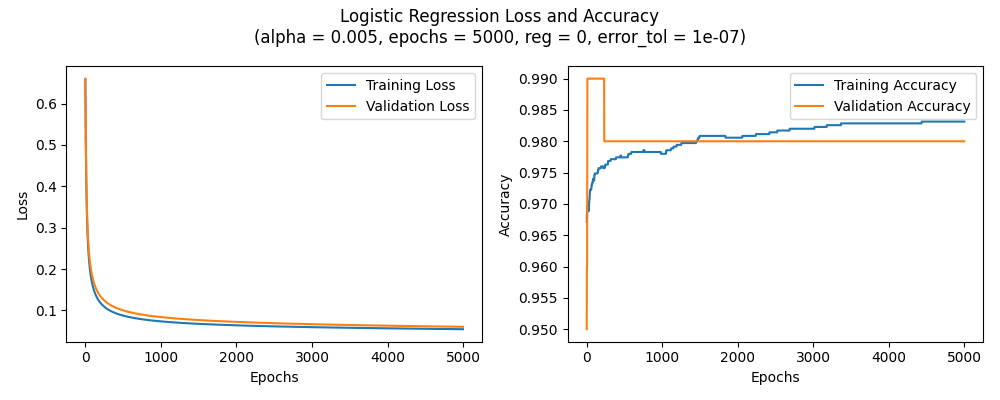
\includegraphics[width=\linewidth]{Figure_1}
	\caption{$\alpha = 0.005$, testing accuracy $ = 97.931\%$}
	\label{fig:plot1}
\end{figure}

\begin{figure}[H]
	\centering
	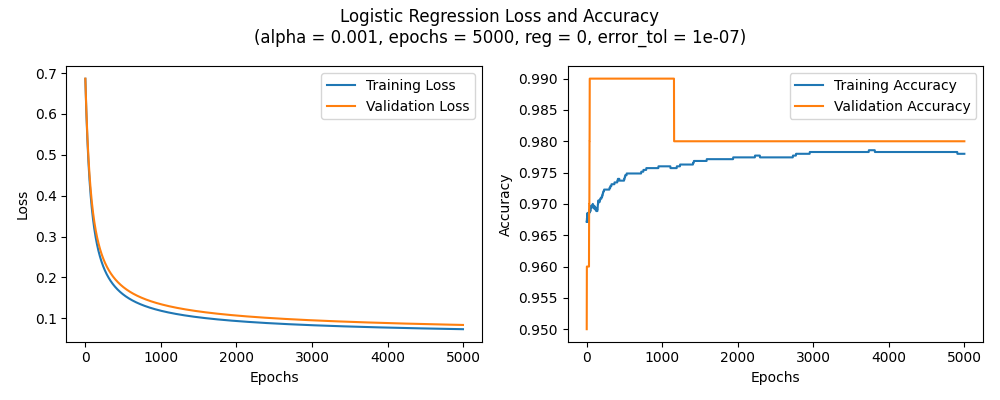
\includegraphics[width=\linewidth]{Figure_2}
	\caption{$\alpha = 0.001$, testing accuracy $ = 97.241\%$}
	\label{fig:plot2}
\end{figure}

\begin{figure}[H]
	\centering
	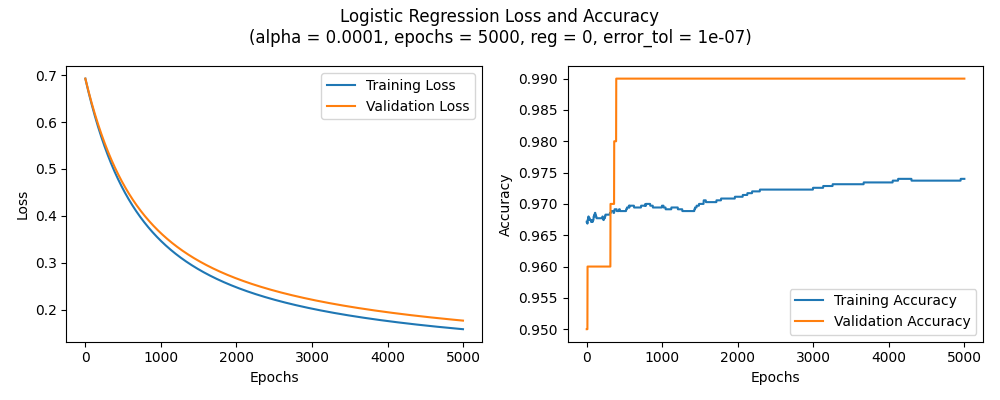
\includegraphics[width=\linewidth]{Figure_3}
	\caption{$\alpha = 0.0001$, testing accuracy $ = 97.241\%$}
	\label{fig:plot3}
\end{figure}

The best learning rate, surprisingly, was $\alpha = 0.005$ as seen in figure \ref{fig:plot1}, which also happened to be the fastest learning rate. Not only did it provide the fastest convergence, but it also provided the best final testing accuracy of $97.931\%$. Despite the other two learning rates generating higher final validation accuracies, the testing accuracy is the true performance measurement of the model, and thus the validation accuracy should not be considered over the testing. 

\subsection{Generalization}

\begin{figure}[H]
	\centering
	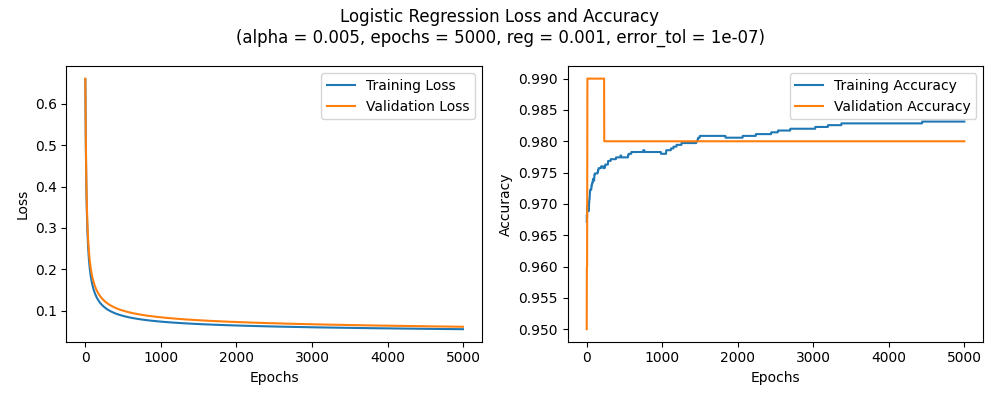
\includegraphics[width=\linewidth]{Figure_4}
	\caption{reg $ = 0.001$, testing accuracy $ = 97.931\%$}
	\label{fig:plot4}
\end{figure}

\begin{figure}[H]
	\centering
	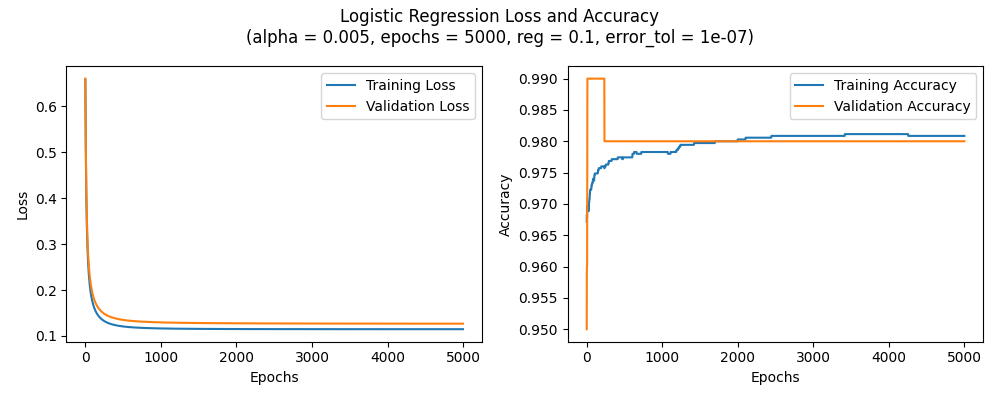
\includegraphics[width=\linewidth]{Figure_5}
	\caption{reg $ = 0.1$, testing accuracy $ = 97.931\%$}
	\label{fig:plot5}
\end{figure}

\begin{figure}[H]
	\centering
	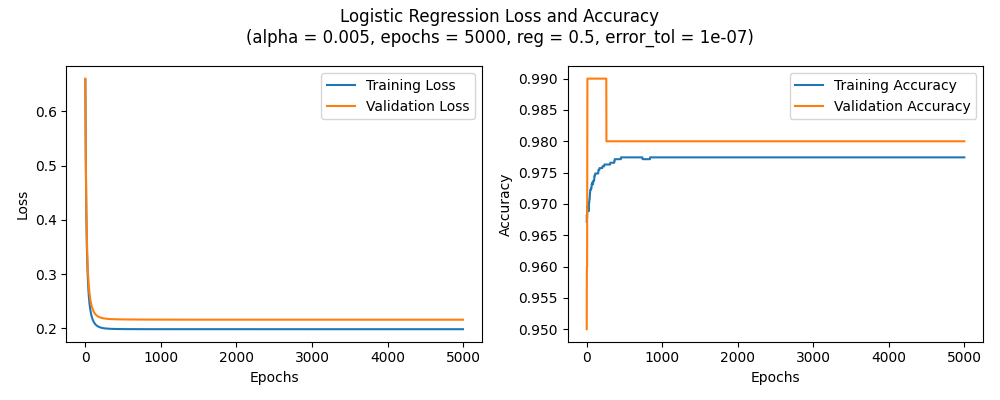
\includegraphics[width=\linewidth]{Figure_6}
	\caption{reg $ = 0.5$, testing accuracy $ = 97.931\%$}
	\label{fig:plot6}
\end{figure}

The regularization parameter $\lambda$ had no effect whatsoever on neither the final testing accuracy nor the validation accuracy of the model. The only noticeable impact was on the training accuracy, which decreased as $\lambda$ increased, and the speed of convergence (i.e. the rate at which the training and validation loss reached asymptotic behaviour), which increased as $\lambda$ increased. The final training accuracies for the three different hyperparameters were $98.314\%$ for figure \ref{fig:plot4}, $98.086\%$ for figure \ref{fig:plot5}, and $97.743\%$ for figure \ref{fig:plot6}.

\newpage

\section{Logistic Regression in TensorFlow}

\textit{I initially attempted to build the TensorFlow model using TensorFlow 2.x, but unfortunately there was not a lot of documentation concerning the migration from the} \texttt{tf.Session()} \textit{and}  \texttt{tf.get\_variable()}\textit{/}\texttt{tf.placeholder()} \textit{infrastructure to the new 2.x} \texttt{tf.GradientTape()}\textit{,} \texttt{tf.Variable()}\textit{, and the function decorator} \texttt{@tf.function}\textit{. For the sake of functionality, I opted to build in TensorFlow 1.x with the following modifications.}

\begin{lstlisting}
import tensorflow.compat.v1 as tf
tf.disable_v2_behavior()
\end{lstlisting}

\subsection{Building the Computational Graph}

\begin{lstlisting}
def buildGraph():
    # Initialize TensorFlow Graph object
    graph = tf.Graph()

    with graph.as_default():
        # Initialize weight and bias tensors
        # Inefficient to import all data to check size for weights, we already know the size will be
        # 28 * 28 = 784 by 1 dimensional tensor, and bias will be a 1 by 1 tensor
        w = tf.Variable(tf.truncated_normal(shape=(28 * 28, 1), mean=0.0, stddev=0.5, dtype=tf.float32))
        b = tf.Variable(tf.zeros(1))

        # Placeholders for data, labels, and reg
        x = tf.placeholder(tf.float32)
        y = tf.placeholder(tf.uint8)
        reg = tf.placeholder(tf.float32)

        # Calculate loss and optimizer
        y_hat = hypothesis(w, b, x)
        loss = tf.losses.sigmoid_cross_entropy(y, y_hat)
        # Hardcode learning rate alpha = 0.001
        optimizer = tf.train.AdamOptimizer(learning_rate=1e-3).minimize(loss)
        _, accuracy = tf.metrics.accuracy(y, y_hat)

    return w, b, x, y, reg, y_hat, loss, optimizer, accuracy, graph
\end{lstlisting}

Although the predicted labels $\hat{y}$ is returned, it was never used. The training accuracy was instead calculated within the graph and its reference was passed to the training function, which was useful for calculating the accuracies for both the validation and testing datasets.

\subsection{Implementing Stochastic Gradient Descent}

\textit{As with the Numpy gradient descent implementation, all the plotting-related sections have been omitted. Below is the simplified code.}

\begin{lstlisting}
def train(w, b, x, y, loss, optimizer, accuracy, graph, batch_size, epochs, reg):
    trainData, validData, testData, trainTarget, validTarget, testTarget = loadData()

    # Flatten all input data into a 1-dimensional vector
    # 28 x 28 tensor becomes a 784-length vector
    trainData = trainData.reshape(len(trainData), -1)
    validData = validData.reshape(len(validData), -1)
    testData = testData.reshape(len(testData), -1)

    d = len(trainData[0])
    N = len(trainTarget)

    with tf.Session(graph=graph) as sess:
        sess.run(tf.local_variables_initializer())
        sess.run(tf.global_variables_initializer())

        # Calculate batch size
        batches = int(N / batch_size)

        for epoch in range(epochs):
            # Shuffle dataset
            indices = np.arange(N)
            np.random.shuffle(indices)
            trainData, trainTarget = trainData[indices], trainTarget[indices]

            for batch in range(batches):
                batch_index = batch * batch_size

                # Run optimizer
                sess.run(optimizer,
                    feed_dict={
                        x : trainData[batch_index:(batch_index + batch_size)], 
                        y : trainTarget[batch_index:(batch_index + batch_size)],
                        reg : 0
                    }
                )
\end{lstlisting}

\begin{figure}[H]
	\centering
	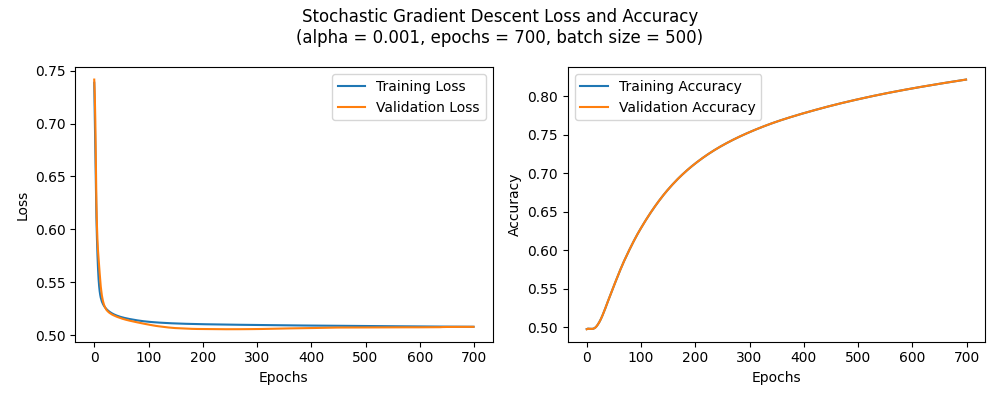
\includegraphics[width=\linewidth]{Figure_7}
	\caption{Batch size $ = 500$, testing accuracy $ = 82.157\%$}
	\label{fig:plot7}
\end{figure}

Although the training was much quicker than the normal gradient descent implemented in Numpy, the model had slightly worse performance on all three datasets. The TensorFlow stochastic gradient descent model has a noticeably more flattened and plateaued training and validation accuracy curve. This is expected behaviour of mini-batch stochastic gradient descent, as batching will introduce noise yet have a regularization effect, still resulting in quick yet effective training. 

\subsection{Batch Size Investigation}

\begin{figure}[H]
	\centering
	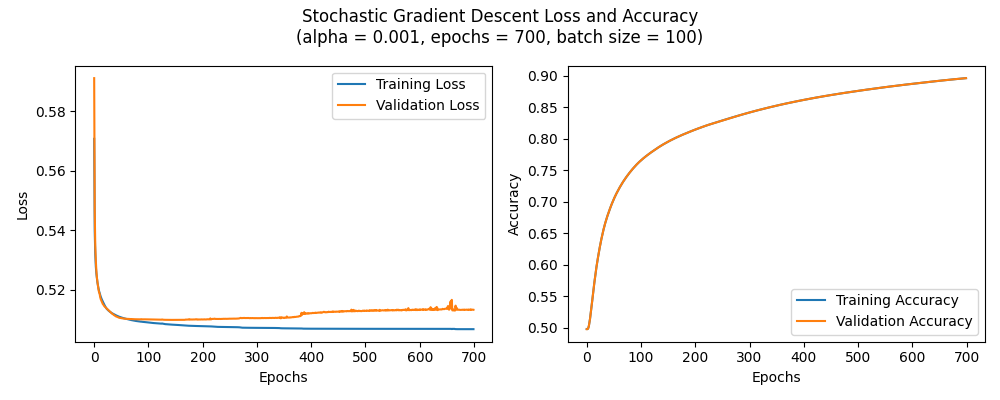
\includegraphics[width=\linewidth]{Figure_8}
	\caption{Batch size $ = 100$, testing accuracy $ = 89.632\%$}
	\label{fig:plot8}
\end{figure}

\begin{figure}[H]
	\centering
	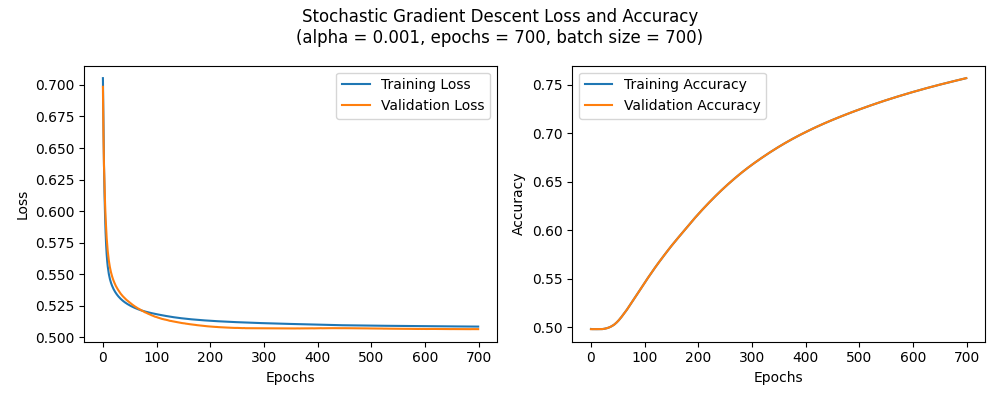
\includegraphics[width=\linewidth]{Figure_9}
	\caption{Batch size $ = 700$, testing accuracy $ = 75.668\%$}
	\label{fig:plot9}
\end{figure}

\begin{figure}[H]
	\centering
	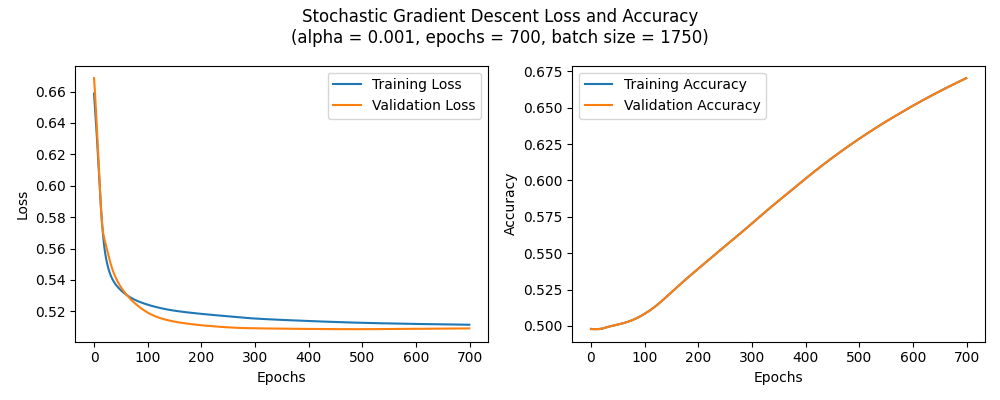
\includegraphics[width=\linewidth]{Figure_10}
	\caption{Batch size $ = 1750$, testing accuracy $ = 67.026\%$}
	\label{fig:plot10}
\end{figure}

As batch sizes increase, the number of batches decrease. Larger batch sizes allow the processor (or GPU) to take full advantage of the optimized parallel vector computations for gradient descent, and thus will have a shorter training speed. This, however, reduces the natural regularization effect that stochastic gradient descent has, and will introduce less noise and have worse generalization. This effect is shown especially on models shown in figure \ref{fig:plot9} and figure \ref{fig:plot10}, as their training and validation accuracy curves are much more linear, and their final testing accuracies are worse: indicating poor generalization and hastened training. In figure \ref{fig:plot8}, the effects of a smaller batch size is clear. The validation loss curve has clear spikes and abnormalities, representing the random noise caused by dataset shuffling and the stochastic nature of the gradient descent. 

\newpage

\subsection{Hyperparameter Investigation}

\begin{figure}[H]
	\centering
	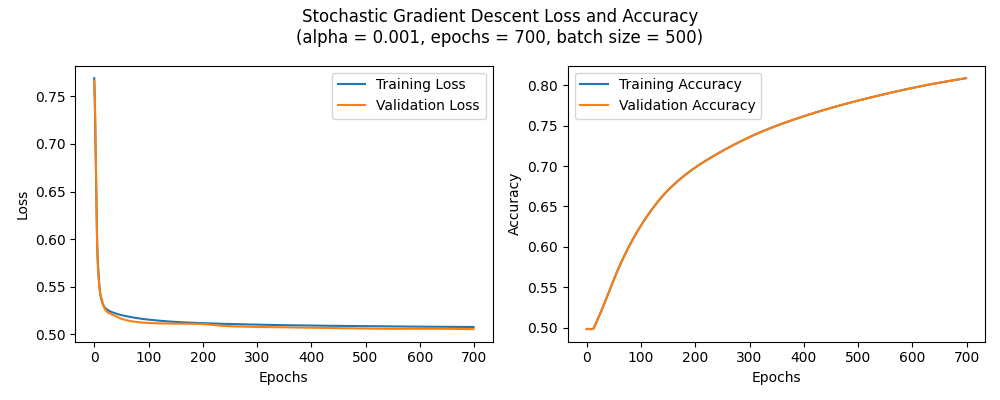
\includegraphics[width=\linewidth]{Figure_11}
	\caption{$\beta_1 = 0.95$, testing accuracy $ = 80.902\%$}
	\label{fig:plot11}
\end{figure}

\begin{figure}[H]
	\centering
	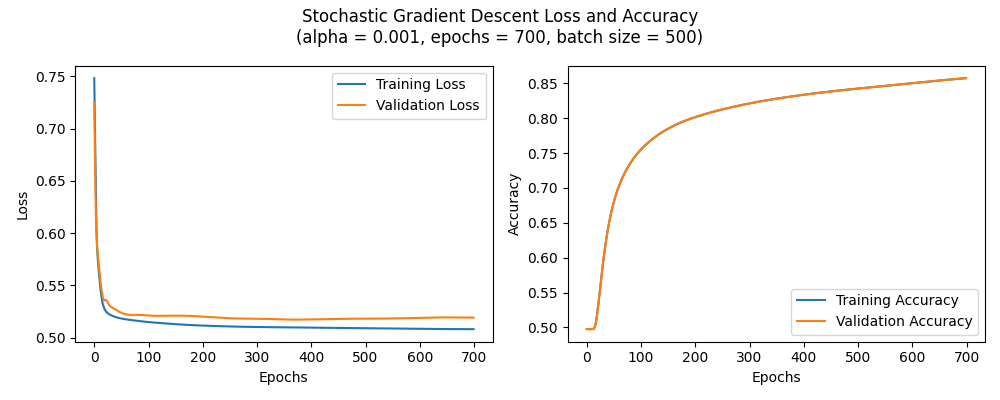
\includegraphics[width=\linewidth]{Figure_12}
	\caption{$\beta_1 = 0.99$, testing accuracy $ = 85.749\%$}
	\label{fig:plot12}
\end{figure}

\begin{figure}[H]
	\centering
	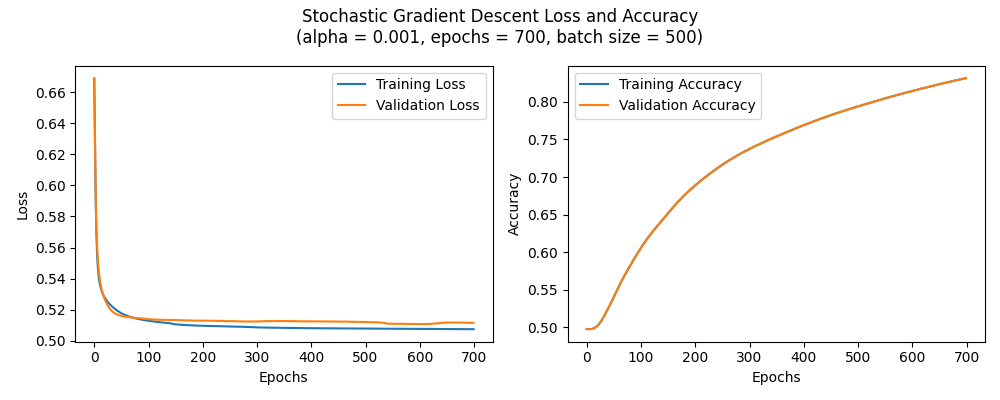
\includegraphics[width=\linewidth]{Figure_13}
	\caption{$\beta_2 = 0.99$, testing accuracy $ = 83.144\%$}
	\label{fig:plot13}
\end{figure}

\begin{figure}[H]
	\centering
	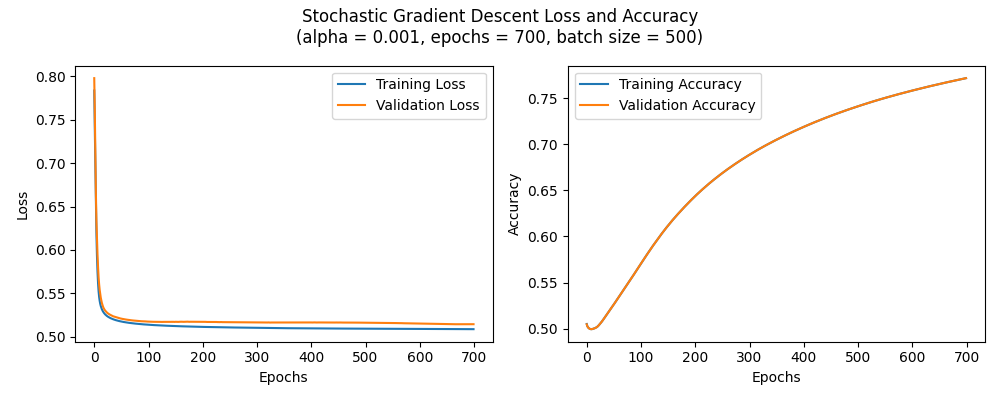
\includegraphics[width=\linewidth]{Figure_14}
	\caption{$\beta_2 = 0.9999$, testing accuracy $ = 77.165\%$}
	\label{fig:plot14}
\end{figure}

\begin{figure}[H]
	\centering
	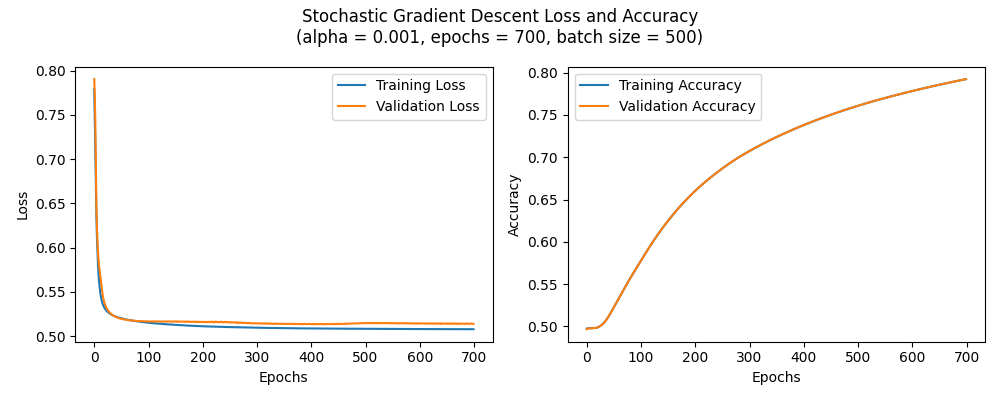
\includegraphics[width=\linewidth]{Figure_15}
	\caption{$\epsilon = 1 \times 10^{-9}$, testing accuracy $ = 79.239\%$}
	\label{fig:plot15}
\end{figure}

\begin{figure}[H]
	\centering
	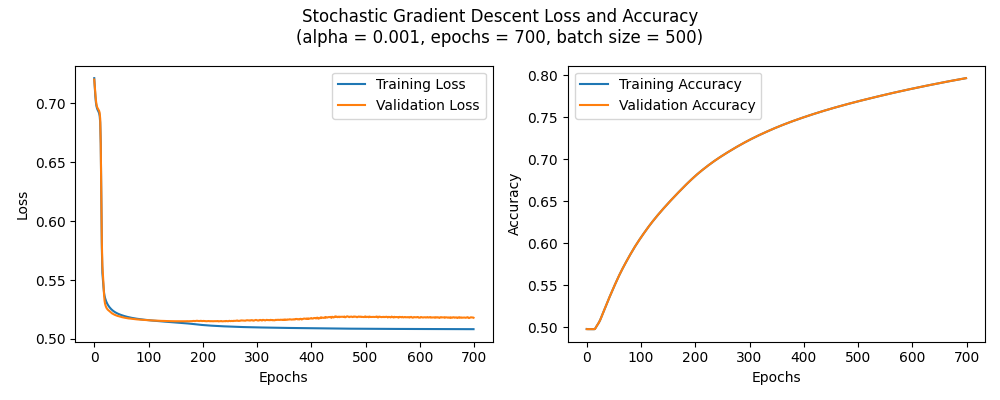
\includegraphics[width=\linewidth]{Figure_16}
	\caption{$\epsilon = 1 \times 10^{-4}$, testing accuracy $ = 79.650\%$}
	\label{fig:plot16}
\end{figure}

\textit{Some of the predicted behaviour of these hyperaparameters are not exhibited is most of the iterations, namely due to the randomness of stochastic gradient descent. The expected behaviour, however, is noted below.}

\begin{enumerate}[label=(\alph*)]
	\item $\beta_1$ controls the first moment in the Adam optimizer. This parameter affects how many historical samples are considered when computing momentum during gradient descent. For example, $\beta_1 = 0.9$ will consider the past $10$ gradients for the momentum in the next descent. As $\beta_1$ increases, the descent will become smoother with less oscillations as it averages over more and more past samples, which could result in worse performance.
	\item $\beta_2$ controls the second moment of \texttt{RMSProp}. Instead of simply calculating the weighted averages of past gradients, $\beta_2$ will compute the squares of the gradients, and perform a bias correction step. Increasing this parameter has a similar effect as $\beta_1$, with the reduction of noise and performance.
	\item $epsilon$ is used to avoid zero-divisions during the gradient descent momentum computations. Although this value is usually kept low as to avoid affecting the weights during the descent, increasing the value can have similar effects as both $\beta_1$ and $\beta_2$ by reducing the noise yet decreasing performance. A value as high as $\epsilon = 1 \times e^{-4}$ can pose heavy influence on the weights, leading to further worsened performance.
\end{enumerate}

\subsection{Comparison against Batch GD}
Although the Adam stochastic gradient descent seems to have faster descent and optimized computations, this came at a cost of worse performance on the testing dataset. The Numpy implementation of batch gradient descent achieved a maximum accuracy of around $\approx 95\%$, while the stochastic gradient descent could only achieve around $\approx 85\%$. The loss curves take a similar shape, but the stochastic gradient descent reached a much higher plateau than the batch gradient descent. 

\end{document}
